% !TeX root = ../main.tex

\newlecture[The Term Structure of Interest Rates][Sep 28, 2026]

\header{The Yield Curve}
In general, yields on bonds of different maturities are different, i.e. \ul{interest rates are a function of time}.
\\Plotting yield vs.\ time to maturity for bonds gives the \rb{yield curve}.

\begin{center}
\begin{tikzpicture}
    \draw[->] (0,0) -- (6,0) node[right] {time to maturity};
    \draw[->] (0,0) -- (0,3) node[above] {yield};
    \draw[thick, domain=0.2:5.3, smooth, variable=\x] plot ({\x}, {2.4 - 1.4*exp(-0.7*\x)});
\end{tikzpicture}
\end{center}

Real U.S.\ Treasury yield curves (yahoo.com): on Sep 10, 2004 the curve rose steeply from about 1.5\% (3 months) to 5\% (30 years); on Oct 4, 2005 it was much flatter, from about 3.5\% to 4.6\%. The \ul{shape of the curve changes over time}.

The yield curve is not exactly what we want, since bonds may have coupons (intermediate cash flows). We would really like to know the interest rate on a \dbb{single cash flow at time $t$}, with no intermediate cash flows.

\begin{center}
\begin{tikzpicture}
    \draw[->] (-0.3,0) -- (5,0);
    \node[below] at (0,-0.1) {$0$};
    \node[below] at (4,-0.1) {$t$};
    \draw[->, thick] (4,0) -- (4,1.2);
\end{tikzpicture}
\end{center}

\header{Spot Rates}
\begin{definition}[Spot Rate]
    Interest rates for a specific time $t$. Always \dbb{annual nominal interest rates}, can be compounded yearly, $m$ periods per year, or continuously.
\end{definition}

\begin{framed}
\begin{center}
\begin{tikzpicture}
    \draw[->] (0,0) -- (6,0) node[right] {time};
    \draw[->] (0,0) -- (0,3) node[above] {spot rate};
    \draw[thick, domain=0.2:5.3, smooth, variable=\x] plot ({\x}, {2.4 - 1.4*exp(-0.7*\x)});
\end{tikzpicture}
\end{center}

Plotting spot rates vs.\ time gives the \rb{spot rate curve}, also known as the \rb{term structure of interest rates}.
\\We can price bonds reliably with predictions through the term structure of interest (quant!!).
\end{framed}


\heading{Present Value and Spot Rates}
When computing present value, the \ul{spot rate corresponding to the time of each cash flow} must be used for discounting:
\[\boxed{PV = x_0 + \frac{x_1}{1+s_1} + \frac{x_2}{(1+s_2)^2} + \cdots + \frac{x_n}{(1+s_n)^n}}\]

\begin{example}
    \begin{center}
    \begin{tikzpicture}
        \draw[->] (-0.3,0) -- (5,0);
        \foreach \x in {0,1,2,3,4} {
            \draw (\x,0.05) -- (\x,-0.05);
        }
        \draw[->, thick] (0,0) -- (0,-0.6) node[below] {$-1$};
        \draw[->, thick] (1,0) -- (1,1.2) node[above] {$2$};
        \draw[->, thick] (2,0) -- (2,0.6) node[above] {$1$};
        \draw[->, thick] (3,0) -- (3,-1.2) node[below] {$-2$};
        \draw[->, thick] (4,0) -- (4,0.6) node[above] {$1$};
    \end{tikzpicture}
    \end{center}
    \begin{center}
    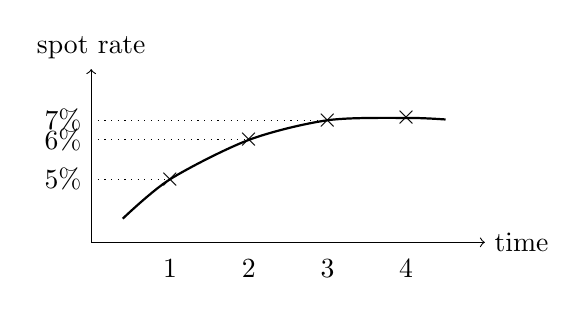
\begin{tikzpicture}
        \draw[->] (0,0) -- (5,0) node[right] {time};
        \draw[->] (0,0) -- (0,2.2) node[above] {spot rate};
        \foreach \x in {1,2,3,4} {
            \node[below] at (\x,-0.1) {\x};
        }
        \draw[thick, smooth] plot coordinates {(0.4,0.3) (1,0.8) (2,1.3) (3,1.55) (4,1.58) (4.5,1.56)};
        \foreach \x/\y/\r in {1/0.8/5, 2/1.3/6, 3/1.55/7} {
            \draw[dotted] (0,\y) -- (\x,\y);
            \node[left] at (0,\y) {\r\%};
        }
        \foreach \x/\y in {1/0.8, 2/1.3, 3/1.55, 4/1.58} {
            \node at (\x,\y) {$\times$};
        }
    \end{tikzpicture}
    \end{center}
    \begin{center}
    \begin{tabular}{lccccc}
        \toprule
        Time & 0 & 1 & 2 & 3 & 4\\
        \midrule
        Cash flow & $-1$ & 2 & 1 & $-2$ & 1\\
        Spot rate & & 5\% & 6\% & 7\% & 7\%\\
        \bottomrule
    \end{tabular}
    \end{center}
    \[PV = -1 + \frac{2}{1.05} + \frac{1}{1.06^2} + \frac{-2}{1.07^3} + \frac{1}{1.07^4} = 0.925\]
\end{example}

\heading{Determining Spot Rates}
If you know the price of a \dbb{zero-coupon bond}, \ul{its yield is the spot rate}. Given price $P$ and face value $F$ of a zero maturing at $t$:
\[\boxed{P = Fe^{-s_t t}} \quad \text{(continuous compounding)} \qquad \boxed{P = \frac{F}{(1+s_t)^t}} \quad \text{(discrete compounding)}\]
\b{Problem}: What if there are no zeros?
\\\b{Solution}: Construct a zero-coupon bond from coupon bonds.

\header{Constructing Zeros}
Take two coupon bonds with the same maturity (and coupon dates) and form a portfolio of $x$ of bond 1 and $y$ of bond 2 (negative means short).

\begin{center}
\begin{tikzpicture}
    \node[left] at (-0.5,0.5) {Bond $i$};
    \draw[->] (-0.3,0) -- (7.5,0);
    \node[above left] at (0,0) {$0$};
    \node[below] at (6.5,0) {maturity};
    \draw[->, thick] (0,0) -- (0,-1) node[below] {$P_i$};
    \draw[->, thick] (1,0) -- (1,0.9) node[above] {$C_i$};
    \draw[->, thick] (2,0) -- (2,0.9) node[above] {$C_i$};
    \draw[->, thick] (3,0) -- (3,0.9) node[above] {$C_i$};
    \draw[->, thick] (4,0) -- (4,0.9) node[above] {$C_i$};
    \node at (5.2,0.4) {$\cdots$};
    \draw[->, thick] (6.5,0) -- (6.5,1.7);
    \node at (6.5,2.3) {$C_i$};
    \node at (6.5,1.95) {$F_i$};
\end{tikzpicture}
\end{center}

Three equations for the portfolio:
\[\boxed{\begin{aligned}
    \text{Coupon:} &\quad xC_1 + yC_2 = C_0 \\
    \text{Face:} &\quad xF_1 + yF_2 = F_0 \\
    \text{Price:} &\quad xP_1 + yP_2 = P_0
\end{aligned}}\]
To construct a zero, set $C_0 = 0$ and $F_0 = \$100$, assuming $F_0 = F_1 = F_2$. Then solve for $x$ and $y$. 
\\The price of the zero is then $P_0 = xP_1 + yP_2$, and the spot rate could be computed.

\begin{example}
    Portfolio of 3 of bond 1 (face \$100, 10\% coupon) and $-2.5$ of bond 2 (face \$100, 12\% coupon), both maturing at $t=5$:
    \begin{center}
    \begin{tabular}{lcccc}
        \toprule
        Time & 0.5 & 1 & $\cdots$ & 5\\
        \midrule
        Bond 1 & 10 & 10 & $\cdots$ & 110\\
        Bond 2 & 12 & 12 & $\cdots$ & 112\\
        Portfolio & 0 & 0 & $\cdots$ & 50\\
        \bottomrule
    \end{tabular}
    \end{center}
    Coupons cancel: $3(10) - 2.5(12) = 0$, leaving only $3(110) - 2.5(112) = 50$ at maturity, a zero.
\end{example}

\begin{example}
    Bond 1: 10 year, 10\% coupon, $P_1 = \$98.72$. Bond 2: 10 year, 8\% coupon, $P_2 = \$85.89$.
    \\(Note: Choose two bonds with the \dbb{same maturity}, so the spot rate for that maturity can be computed)
    \\Create a zero:
    \[\begin{cases}
        \text{Coupon:} & 10x + 8y = 0\\
        \text{Face:} & 100x + 100y = 100
    \end{cases} \quad \Rightarrow \quad x = -4,\ y = 5\]
    Price of zero: $xP_1 + yP_2 = -4(98.72) + 5(85.89) = \$34.57$
    \\Spot Rate (discrete compounding):
    \[34.57 = \frac{100}{(1+s_{10})^{10}} \quad \Rightarrow \quad s_{10} = 0.112 = 11.2\%\]
    Note: if possible, you can compare this computed value with the actual yield, then see which one is "better"
\end{example}

\header{Forward Rates}
\begin{definition}[\rb{Forward Rates}]
    The interest rate for money to be borrowed between two dates \ul{in the future}, but under terms \ul{agreed upon today}. 
    \[f_{t_1,t_2}: \text{the forward rate between $t_1$ and $t_2$.}\]
    Note: $t_1$ can be 0, but not negative, when $t_1 = 0$, $f_{0, t_2} = $ to the spot rate of $t_2$.
\end{definition}
How can forward rates be computed from the spot rate curve?

Starting with \$1 at time 1 and moving it to time 2, we should have $1+f_{1,2}$ by the definition of the forward rate. Spot rates tell us how to move money to and from time 0, so we can instead go \ul{through time 0}:

\begin{center}
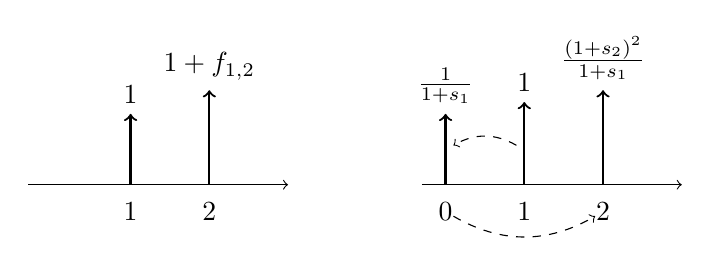
\begin{tikzpicture}
    % direct
    \draw[->] (-0.3,0) -- (3,0);
    \node[below] at (1,-0.1) {$1$};
    \node[below] at (2,-0.1) {$2$};
    \draw[->, thick] (1,0) -- (1,0.9) node[above] {$1$};
    \draw[->, thick] (2,0) -- (2,1.2) node[above] {$1+f_{1,2}$};
    % via time 0
    \begin{scope}[xshift=5cm]
        \draw[->] (-0.3,0) -- (3,0);
        \node[below] at (0,-0.1) {$0$};
        \node[below] at (1,-0.1) {$1$};
        \node[below] at (2,-0.1) {$2$};
        \draw[->, thick] (0,0) -- (0,0.9) node[above] {$\frac{1}{1+s_1}$};
        \draw[->, thick] (1,0) -- (1, 1.05) node[above] {$1$};
        \draw[->, thick] (2,0) -- (2,1.2) node[above] {$\frac{(1+s_2)^2}{1+s_1}$};
        \draw[->, dashed] (0.9,0.5) to[bend right] (0.1,0.5);
        \draw[->, dashed] (0.1,-0.4) to[bend right] (1.9,-0.4);
    \end{scope}
\end{tikzpicture}
\end{center}

\[1+f_{1,2} = \frac{(1+s_2)^2}{1+s_1} \quad \Rightarrow \quad \boxed{f_{1,2} = \frac{(1+s_2)^2}{1+s_1} - 1}\]

\begin{example}
    Spot rates for 1 and 2 years are 7\% and 8\%. The implied forward rate is
    \[f_{1,2} = \frac{(1.08)^2}{1.07} - 1 = 0.0901\]
    Note that the forward rate has to be \dbb{larger} than 8\% to balance out the \((1+0.0.8)^2\)
\end{example}

\heading{Formula for Forward Rates}
Invest \$1 at time 0 until time $j$ in two ways: (1) at the spot rate $s_i$ until $i$, then at the forward rate $f_{i,j}$ until $j$; (2) directly at the spot rate $s_j$. Both must give the same result:

\begin{center}
\begin{tikzpicture}
    % (1) via time i
    \node at (1.6,1.6) {(1) through $i$};
    \foreach \row/\t/\h/\lab in {0/0/0.8/{$1$}, -1.9/1.5/0.8/{$(1+s_i)^i$}, -3.8/3/0.8/{$(1+s_i)^i(1+f_{i,j})^{j-i}$}} {
        \begin{scope}[yshift=\row cm]
            \draw[->] (-0.3,0) -- (4,0);
            \node[below] at (0,-0.05) {$0$};
            \node[below] at (1.5,-0.05) {$i$};
            \node[below] at (3,-0.05) {$j$};
            \draw[->, thick] (\t,0) -- (\t,\h) node[above] {\lab};
        \end{scope}
    }
    \draw[->, dashed] (0.3,-0.5) -- (1.2,-1.1);
    \draw[->, dashed] (1.8,-2.4) -- (2.7,-3.0);
    % divider
    \draw[blue] (5.2,1.8) -- (5.2,-4.3);
    % (2) direct
    \begin{scope}[xshift=6.4cm]
        \node at (1.6,1.6) {(2) directly};
        \foreach \row/\t/\lab in {0/0/{$1$}, -3.8/3/{$(1+s_j)^j$}} {
            \begin{scope}[yshift=\row cm]
                \draw[->] (-0.3,0) -- (4,0);
                \node[below] at (0,-0.05) {$0$};
                \node[below] at (1.5,-0.05) {$i$};
                \node[below] at (3,-0.05) {$j$};
                \draw[->, thick] (\t,0) -- (\t,0.8) node[above] {\lab};
            \end{scope}
        }
        \draw[->, dashed] (0.3,-0.5) -- (2.7,-3.0);
    \end{scope}
\end{tikzpicture}
\end{center}
\[\boxed{(1+s_i)^i(1+f_{i,j})^{j-i} = (1+s_j)^j} \qquad f_{i,j} = \left[\frac{(1+s_j)^j}{(1+s_i)^i}\right]^{1/(j-i)} - 1\]
Note: this calculation must be \ul{consistent with the type of compounding}.

\begin{example}
    Spot rates for 2 and 6 years are 3\% and 5\%. The implied forward rate is
    \[(1+s_2)^2(1+f_{2,6})^4 = (1+s_6)^6 \quad \Rightarrow \quad f_{2,6} = \left(\frac{(1.05)^6}{(1.03)^2}\right)^{1/4} - 1 = 6.01\%\]
\end{example}

\begin{definition}
    Rates that span only 1 period are \rb{short rates}. E.g.\ for yearly compounding: $s_1, f_{1,2}, f_{2,3}, \dots$
\end{definition}
Short rates can be determined from the spot rate curve and vice versa.

\header{Term Structure Explanations}
Why isn't the term structure (spot rate curve) flat? Three explanations:
\begin{enumerate}[label=(\arabic*)]
    \item \b{Expectations Theory}: spot rates are determined by the expectations of what interest rates will be. E.g.\ if the spot rate curve slopes upward, it is because people expect interest rates to increase in the future.
    \item \b{Liquidity Preference}: investors prefer short term securities over long term ones, since long term securities ``tie up'' money for long. There are also secure investments that are both easy to get in and out of.
    \item \b{Market Segmentation}: the fixed income market is segmented by maturity dates. The rate for each maturity is determined by the group of investors interested in that maturity, i.e.\ simple supply and demand among those investors.
\end{enumerate}

\header{Expectation Dynamics}
Forward rates are rates in the future that are agreed upon \rb{now}. But we don't know what the \dbb{actual future rates} will be when that time arrives, since spot rate curves could change.
When forward rates are used as a prediction (could be wrong) of the actual future rates, this forecast is called \rb{expectation dynamics}.
\\Prohibits arbitrage, using forward rates that are anchored on the spot rates today.

\heading{The Invariance Theorem}
If interest rates evolve according to expectation dynamics, then a sum of money invested in the interest rate market for $n$ years, will grow by a factor of $(1+s_n)^n$ \ul{regardless of the investment and reinvestment strategy} (no matter what combination of spot and forward rates).

\begin{center}
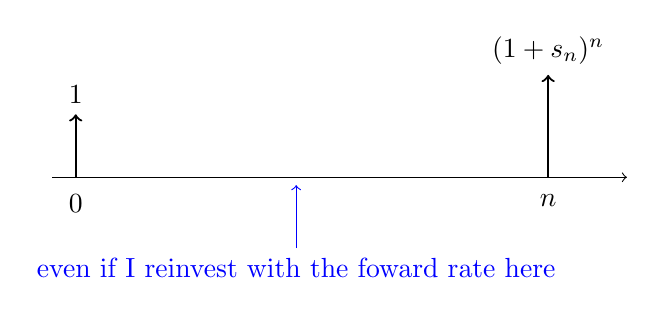
\begin{tikzpicture}
    \draw[->] (-0.3,0) -- (7,0);
    \node[below] at (0,-0.1) {$0$};
    \node[below] at (6,-0.1) {$n$};
    \draw[->, thick] (0,0) -- (0,0.8) node[above] {$1$};
    \draw[->, thick] (6,0) -- (6,1.3) node[above] {$(1+s_n)^n$};
    \draw[->, blue] (2.8,-0.9) -- (2.8,-0.1);
    \node[blue, below] at (2.8,-0.9) {even if I reinvest with the foward rate here};
\end{tikzpicture}
\end{center}

\b{Why?} Implied forward rates were \ul{computed to satisfy exactly this relationship}.
\\So even if you don't lock in a future interest rate now, you can still use forward rates for discounting, \ul{as long as you assume expectation dynamics}.


If expectation dynamics are assumed, the invariance thoerem is true (will always equal the same return value regardless of investment strategies.)